\documentclass[10pt,a4paper,twocolumn,twoside]{article}
\usepackage[utf8]{inputenc}
\usepackage[catalan]{babel}
\usepackage{multicol}
\usepackage{graphicx}
\usepackage{fancyhdr}
\usepackage{times}
\usepackage{titlesec}
\usepackage{url}
\usepackage{multirow}
\usepackage{tabularx}
\usepackage{lettrine}
\usepackage[top=2cm, bottom=1.5cm, left=2cm, right=2cm]{geometry}
\usepackage[figurename=Fig.,tablename=TAULA]{caption}
\usepackage{mathtools}
\usepackage{placeins}
\usepackage{float}
\usepackage{array}
\usepackage{subcaption}
\usepackage{multicol,lipsum}
\usepackage[export]{adjustbox}
\expandafter\def\expandafter\UrlBreaks\expandafter{\UrlBreaks%  save the current one
  \do\a\do\b\do\c\do\d\do\e\do\f\do\g\do\h\do\i\do\j%
  \do\k\do\l\do\m\do\n\do\o\do\p\do\q\do\r\do\s\do\t%
  \do\u\do\v\do\w\do\x\do\y\do\z\do\A\do\B\do\C\do\D%
  \do\E\do\F\do\G\do\H\do\I\do\J\do\K\do\L\do\M\do\N%
  \do\O\do\P\do\Q\do\R\do\S\do\T\do\U\do\V\do\W\do\X%
  \do\Y\do\Z}
\captionsetup[table]{textfont=sc}

\author{\LARGE\sffamily Miquel Freixes Faya}
\title{\Huge{\sffamily Anàlisis de la relació entre les emissions de gasos hivernacle i l'augment de la temperatura mitjançant algorismes i tecnologies de Big Data}}
\date{}

\newcommand\blfootnote[1]{%
  \begingroup
  \renewcommand\thefootnote{}\footnote{#1}%
  \addtocounter{footnote}{-1}%
  \endgroup
}

%
%\large\bfseries\sffamily
\titleformat{\section}
{\large\sffamily\scshape\bfseries}
{\textbf{\thesection}}{1em}{}

\begin{document}

\fancyhead[LO]{\scriptsize MIQUEL FREIXES FAYA: Anàlisis de la relació entre les emissions de gasos hivernacle i l'augment de la temperatura}
\fancyhead[RO]{\thepage}
\fancyhead[LE]{\thepage}
\fancyhead[RE]{\scriptsize EE/UAB TFG INFORMÀTICA: Anàlisis de la relació entre les emissions de gasos hivernacle i l'augment de la temperatura}

\fancyfoot[CO,CE]{}

\fancypagestyle{primerapagina}
{
   \fancyhf{}
   \fancyhead[L]{\scriptsize TFG EN ENGINYERIA INFORMÀTICA, ESCOLA D'ENGINYERIA (EE), UNIVERSITAT AUTÒNOMA DE BARCELONA (UAB)}
   \fancyfoot[C]{\scriptsize Febrer de 2019, Escola d'Enginyeria (UAB)}
}

%\lhead{\thepage}
%\chead{}
%\rhead{\tiny EE/UAB TFG INFORMÀTICA: TÍTOL (ABREUJAT SI ÉS MOLT LLARG)}
%\lhead{ EE/UAB \thepage}
%\lfoot{}
%\cfoot{\tiny{February 2015, Escola d'Enginyeria (UAB)}}
%\rfoot{}
\renewcommand{\headrulewidth}{0pt}
\renewcommand{\footrulewidth}{0pt}
\pagestyle{fancy}

%\thispagestyle{myheadings}
\twocolumn[\begin{@twocolumnfalse}

%\vspace*{-1cm}{\scriptsize TFG EN ENGINYERIA INFORMÀTICA, ESCOLA D'ENGINYERIA (EE), UNIVERSITAT AUTÒNOMA DE BARCELONA (UAB)}

\maketitle

\thispagestyle{primerapagina}
%\twocolumn[\begin{@twocolumnfalse}
%\maketitle
%\begin{abstract}
\begin{center}
\parbox{0.915\textwidth}
{\sffamily
\textbf{Resum--}
L'emissió de gasos hivernacle per part de la humanitat ha estat afectant negativament les temperatures del planeta i augmentant l'efecte del canvi climàtic. L'impacte és tan elevat que les conseqüències són molt visibles actualment: Cada cop hi ha temperatures més elevades, més desertització... Al llarg del temps s'han fet múltiples estudis demostrant i explicant que el canvi climàtic és un fet i que cal actuar immediatament, però encara hi ha molta gent reticent a admetre que existeix aquest canvi climàtic. El principal objectiu d'aquest treball és fer una comparativa de les temperatures de múltiples països i trobar una relació entre aquestes i les emissions de gasos hivernacle. Per fer-ho, es crearà un conjunt de dades, a partir de dades ja existents, i s'entrenarà diversos models d'aprenentatge automàtic per veure si a partir de les emissions es poden predir les temperatures. Aprofitant aquesta comparativa també es pretén avaluar cada un dels algorismes escollits i veure quins aconsegueixen millors resultats.
\\
\\
\textbf{Paraules clau-- } Aprenentatge Computacional, Big Data, Canvi climàtic, Random Forest,  Regressió, Xarxes Neuronals \\
\\
%\end{abstract}
%\bigskip
%\begin{abstract}
\bigskip
\\
\textbf{Abstract--} The release of greenhouse gases by the humanity it is influencing in a negative way the temperatures of the planet and increasing the effect of the climate change. The magnitude of this impact is such that the temperatures are constantly increasing, there is more desertification... Over time there has been multiple studies proving and explaining that climate change is a fact and that we have to act against as soon as possible. But there are people that still don't believe in the existence of it. The main purpose of this project is to do a comparative of the temperatures in multiple countries and find a relationship between them and the greenhouse emisions. To do it, the first step is to create a DataSet, with data that already exists, and train multiple regresion algorithms in order to see if they can predict the temperatures with the emisions. Taking advantage of this situation the project will evaluate each algorithm and try to see if the simple ones are better or it is the other way. 
\\
\\
\textbf{Keywords-- } Machine learning, Big Data, Climate Change, Neural Networks, Random Forest, Regresion\\
}

\bigskip

{\vrule depth 0pt height 0.5pt width 4cm\hspace{7.5pt}%
\raisebox{-3.5pt}{\fontfamily{pzd}\fontencoding{U}\fontseries{m}\fontshape{n}\fontsize{11}{12}\selectfont\char70}%
\hspace{7.5pt}\vrule depth 0pt height 0.5pt width 4cm\relax}

\end{center}


%\end{abstract}
\end{@twocolumnfalse}]

\blfootnote{$\bullet$ E-mail de contacte: m.freixes.faya@gmail.com}
\blfootnote{$\bullet$ Menció realitzada: Tecnologies de la Informació}
\blfootnote{$\bullet$ Treball tutoritzat per: Jordi Casas Roma (DEIC)}
\blfootnote{$\bullet$ Curs 2018/19}
\section{Introducció}
\lettrine[lines=3]{E}{n} els últims anys la temperatura de la Terra no ha parat d'augmentar en la majoria de la seva superfície, efecte resultant del canvi climàtic. Alguns estudis demostren que des del 1980 hi ha hagut un increment d'1 ºC en la temperatura de tota la Terra [1]. Encara que 1 ºC no sembli significant s'ha de contextualitzar, cal incidir en el fet que s'està parlant sobre tota la superfície terrestre, inclosos oceans, per tant que augmenti 1ºC significa que el canvi de temperatura s'ha vist reflectit en l'aigua, els pols, els deserts, etc. Les conseqüències d'aquest fet ja s'estan fent evidents en molts indrets: Hi ha desertització en molts països, els pols s'estan desfent a un ritme alarmant...

S'ha demostrat en múltiples estudis que aquests fets tenen diferents causes que els originen i que una de les més preocupants és la contaminació produïda pels éssers humans. Dins d'aquesta contaminació tenen un paper molt important les emissions dels gasos hivernacle. Aquests gasos sempre han estat presents en l'atmosfera, però des de la revolució industrial la seva presència en l'atmosfera s'ha vist incrementada enormement. Això provoca que les radiacions solars travessin l'atmosfera i que la superfície les absorbeixi. Actualment hi ha molts estudis sobre aquestes emissions i hi ha moltes dades de sensors que han anat registrant les emissions de cada país al llarg dels anys. Al mateix temps, hi ha molts conjunts de dades sobre les temperatures mitjanes mensuals de cada país des de fa anys. Es podria trobar alguna relació entre les emissions de gasos hivernacle i les temperatures per poder predir les temperatures dels pròxims anys? A partir de les emissions i diverses temperatures anteriors, un algorisme seria capaç de predir les temperatures dels pròxims mesos? Aquestes són les preguntes que han motivat aquest treball.

Aquest document està dividit en diverses seccions. A la secció 2 s'expliquen els objectius del treball. A la  secció 3 s'explica l'estat de l'art sobre les tècniques de \textit{machine learning} (ML) i en la 4 la metodologia que s'ha seguit al llarg del treball. Per acabar, a la secció 5 està explicat el desenvolupament, seguidament de l'anàlisi de resultats a la secció 6. Per acabar a la secció 7 s'exposen les conclusions i a la secció 8 s'indiquen les propostes per futurs treballs.   
\section{Objectius}
L'objectiu principal d'aquest treball és analitzar el comportament de diferents algorismes de \textit{machine learning} a l'hora de predir la temperatura d'un país a partir de les seves emissions de gasos hivernacle. Aquest objectiu es limitarà als països del continent d'Europa i al període comprès entre els anys del 1990 al 2012. L'objectiu principal es pot desglossar en diferents subobjectius que s'han d'aconseguir per arribar a satisfer-lo:
\begin{itemize}
\item Crear un conjunt de dades que relacioni els països amb les seves temperatures i les seves emissions, a partir de dades extretes de fonts fiables i lliures de drets. Aquest ha de tenir les suficients dades per poder entrenar els algorismes de ML apropiadament.
\item Analitzar quins són els algorismes de ML més utilitzats actualment en problemes de regressió i conèixer els seus avantatges i inconvenients.
\item Conèixer els paràmetres i trobar la millor configuració de cada un d'ells aplicant mètodes utilitzats en Big Data, com el \textit{grid search} o el \textit{randomized search}.
\item Poder determinar el millor algorisme dels diversos seleccionats i poder extreure els diferents resultats i conclusions de forma gràfica i entenedora.  
\end{itemize}
\section {Estat de l'art}
En aquests darrers anys el \textit{big data} ha passat a ser un dels termes més utilitzats en molts àmbits més enllà de la informàtica, com per exemple, la medicina o l'economia. Aquest concepte s'ha començat a utilitzar degut a l'increment de la complexitat i de la mida dels conjunt de dades, junt amb la necessitat d'un temps de resposta molt baix. Per tot això, els tractaments de dades tradicionals s'han quedat desfasats i hi han hagut d'aparèixer nous paradigmes, algorismes i tecnologies per substituir-los i poder satisfer totes les noves característiques, també conegudes com les 4 V's [2]. Aquestes són el volum, la varietat, la veracitat i la velocitat. Aquest és el context en què entra en joc el \textit{machine learning} i el \textit{deep learning}. 

Una de les eines que actualment s'utilitza molt, pel processament dels conjunts de dades que es consideren dins del \textit{big data}, és el framework Spark. Aquest és un entorn per al processament de dades distribuïdes, que intenta millorar les febleses que té el MapReduce. Aquest entorn és ideal per treballar en entorns distribuïts, ja que és compatible amb tots els serveis que formen part de l'ecosistema d'Apache Hadoop [3].

El \textit{machine learning} és una aplicació de la intel·ligència artificial que dóna a un sistema l'habilitat per poder aprendre a partir de l'experiència. Per aconseguir una bona predicció del sistema cal tenir un conjunt de dades suficientment gran com per poder entrenar-lo i després tenir dades per posar-lo a prova. Per tant, el disseny d'aquests conjunts de dades també és molt important. En aquest aspecte actualment s'utilitza molt la llibreria de Pandas\footnote{\url{https://pandas.pydata.org/}}. Aquesta és una llibreria de codi obert que ofereix estructures de dades molt optimitzades pel seu processament, a més és escalable i fàcil d'entendre.

El \textit{deep learning} és una àrea dins del \textit{machine learning} que està formada per un conjunt d'algorismes destinats a fer anàlisis predictives a partir de la intel·ligència artificial. Actualment, l'API de TensorFLow es la tecnologia més utilitzada a l'hora de programar algorismes de \textit{deep learning}. En canvi, la llibreria de de Scikit-Learn es ideal per començar a familiaritzar-se amb els algorismes, a causa de la seva simplicitat. L'API de TensorFlow és de codi obert i ha estat desenvolupada per Google per tal de construir xarxes neuronals. Aquesta eina permet aprofitar al màxim els recursos locals d'un ordinador, tant CPU com GPU. TensorFlow representa càlculs en forma de grafs, cada node realitza una operació sobre diversos valors, matrius o vectors i com a resultat retorna un tensor. La principal característica que el fa tan utilitzat és que permet l'ús de GPU, la qual cosa aporta un increment important del rendiment en l'entrenament de les xarxes. Aquesta eina té diverses implementacions en diferents llenguatges com C++, Java o Python [3].


\section {Metodologia}
A l'hora de fer projectes hi ha un gran nombre de metodologies per escollir, però en l'àmbit de la informàtica les més utilitzades són les Agile. Això és degut a l'increment del nombre de projectes àgils acabats amb èxit, respecte dels projectes on s'han aplicat les metodologies tradicionals [4]. Dins de la metodologia àgil hi ha diverses metodologies, com Scrum, Kanban, XP, etc. En aquest treball se seguirà la Kanban, a causa del fet que la metodologia Scrum no es podria aprofitar al màxim amb només una persona en el projecte. La principal raó per no escollir Scrum ha estat que molts papers els hauria de fer la mateixa persona, com el de Scrum Master, Product Owner... En conseqüència, algunes de les principals característiques no tindrien sentit [5].

Kanban es basa en una taula de progrés que indica les tasques per fer, les que s'estan fent i les fetes. Això permetrà un seguiment constant de com avança el projecte. També permet treballar segons prioritats, no per temps, i això s'ajusta molt bé al tipus de projecte que es desenvoluparà. A causa del fet que el projecte està format per tasques que es poden paral·lelitzar, i d'altres que cal desenvolupar en serie, apareixeran prioritats al llarg del desenvolupament [6].

La fase del projecte destinada a l'anàlisi dels conjunts de dades es farà utilitzant el software d'Apache Spark a partir de Databricks\footnote{\url{https://databricks.com/}}. S'ha escollit Databricks perquè ofereix un petit clúster amb 6GB de RAM per estudiants, uns recursos suficients per processar el volum de dades desitjat.
A part d'això, tot el progrés de cada etapa s'anirà guardant en un repositori de codi font per tal poder mantenir un històric dels canvis\footnote{\url{ https://github.com/miky96/TFG}}. En el repositori es guardarà els informes, els codis i algorismes necessaris i els conjunt de dades amb les dades.

Finalment es farà servir el llenguatge Python per aquest treball ja que aquest llenguatge és molt utilitzat a l'hora de treballar amb algorismes de \textit{machine learning}. A més, s'utilitzaran algorismes de la llibreria de Scikit Learn\footnote{\url{https://scikit-learn.org/stable/}}, a causa de la gran varietat d'algorismes que ofereix i a la facilitat per implementar-los. No obstant això, el desenvolupament de les xarxes neuronals es farà utilitzant Keras\footnote{\url{https://keras.io/}}. Keras permet treballar amb més detall la implementació de les xarxes i és una API que treballa sobre TensorFlow, per tant es troba en l'estat de l'art de l'àmbit del \textit{deep learning} i es l'eina més adequada per fer xarxes neuronals.
\section {Desenvolupament}
\subsection{Comprensió de les dades}
Al començament, s'han obtingut dos conjunts de dades:

El primer està format de quatre columnes, tal com es mostra a la taula 1:
\begin{enumerate}
\item La \textbf{data}, en format String amb dies mesos i anys.
\item La \textbf{temperatura} mesurada amb un marge d'error del 95\%, serà el valor que es donarà per vàlid al llarg del treball. 
\item El \textbf{nom del país} al qual s'està mesurant les temperatures.
\item El \textbf{marge d'error} que pot tenir la temperatura de la segona columna.
\end{enumerate}
Aquest conjunt de dades està extret de Kaggle\footnote{\url{https://www.kaggle.com/}}, però és una recopilació d'investigacions fetes per Berkeley Earth [7], que és una empresa sense ànim de lucre destinada a revisar i documentar l'increment de temperatura al llarg dels anys. Aquest conjunt de dades és una compressió de dades extretes de més d'1,6 bilions de registres entre els anys 1750 i el 2013 de tot el món per cada mes de l'any.

\begin{table}[th]
\caption{Taula de temperatures}
\begin{center}
\begin{tabular}{  m{1.6cm}| m{0.8cm}| m{1.3cm} | m{2.5cm} }
\hline\hline %inserts double horizontal lines
\textbf{Camp} & \textbf{Tipus} & \textbf{Exemple} & \textbf{Significat} \\
\hline
Data & Date & DD-MM-YYYY & Primer dia de cada mes \\
\hline
Temperatura Mitjana & Float & 2.245 & Temperatura amb una confiança del 95 \%  \\
\hline
País & String & Germany & Nom de cada país \\
\hline
Incertessa & Float & 1.1 & Error del 5 \% de la temperatura\\
\hline
\hline
\end{tabular}
\end{center}
\end{table}

El detall de les dades del segon conjunt es pot veure a la figura 2 i es descriu a continuació:
\begin{enumerate}
\item El \textbf{nom del país} on s'està mesurant.
\item \textbf{L'any} on s'ha mesurat, aquest cop en format d'enter
\item El \textbf{valor de la mitjana} de Kilotones de gas produït per capita en el país
\item El \textbf{tipus de gas} que s'ha mesurat i quins paràmetres s'han utilitzat per fer-ho
\end{enumerate}

D'aquest conjunt de dades s'han extret les dades de les emissions de cada país, dels diferents gasos hivernacle des de l'any 1990 al 2017 [8]. La majoria de mesures estan extretes sense considerar les activitats d'ús de la Terra o d'intercanvi de recursos amb la terra, anomenades en anglès com a LULUCF (\textit{Land Use, Land-Use Change and Forestry}). Bàsicament aquestes activitats comprenen alguns sectors de l'agricultura i/o obtenció de matèries primeres [9]. Aquestes activitats representen un 7\% del total d'emissions, per tant s'analitzarà en el treball el 93\% restant que representa tots els altres sectors com el de la indústria, el turisme i el consum particular, entre d'altres [10].

\begin{table}[th]
\caption{Taula de gasos}
\begin{center}
\begin{tabular}{  m{1.2cm} | m{0.8cm}| m{1.4cm}| m{2.8cm} }
\hline\hline %inserts double horizontal lines
\textbf{Camp} & \textbf{Tipus} & \textbf{Exemple} & \textbf{Significat} \\
\hline
País & String & Belgium & Nom de cada país \\
\hline
Any & Int & 1990 & Any de les dades \\
\hline
Valor & Int & 393126.94 & Mitjana de Kilotones produïdes \\
\hline
Categoria & String & Co2\_lulucf  & Tipus de gas\\
\hline
\hline
\end{tabular}
\end{center}
\end{table}

\subsection{Eines de preprocessament}
Un cop descrits els conjunts de dades es pot començar amb el seu tractament. Per fer aquest pas s'ha utilitzat l'eina de Databricks\footnote{\url{https://databricks.com/}}, optimitzada per treballar amb Spark, a més de permetre treballar amb Pandas i d'altres frameworks o llibreries de processament de dades. Aquesta eina proporciona un clúster amb un màxim de 6GB de RAM. S'ha preferit utilitzar aquesta opció, ja que ha evitat tot el procés d'instal·lar un sistema en una màquina per treballar amb Spark, permetent dedicar més temps al processament de les dades. En aquesta eina s'ha utilitzat el \textit{framework} de pySpark, que és una llibreria per accedir a Spark des del llenguatge Python. El llenagutge natiu de Spark és Scala, però existeixen llibreries per accedir des de diferents llenguatges, com ara Java o Python. A més s'han utilitzat diverses llibreries com Pandas, Numpy i SciPy.

Per una banda tenim Pandas\footnote{\url{https://pandas.pydata.org/}}, una llibreria de codi obert amb llicència de \textit{Berkeley Distributed Systems} optimitzada per al processament de grans volums de dades. Aquesta està integrada en Python i sol ser molt utilitzada per manipulació de dades en aquest llenguatge. Aquesta llibreria proporciona estructures de dades que són flexibles i ràpides que permeten treballar amb elles d'una forma fàcil i intuitiva. El seu element bàsic és el \textit{DataFrame}, que es pot representar com una taula amb files i columnes. Aquest element és molt més fàcil i eficient que un diccionari o una llista gràcies al fet que no cal implementar estructures de bucles molt complicades per anar iterant sobre els seus valors.

Per l'altra banda tenim Spark, un entorn derivat de projectes per a processament de dades masives, com Apache Haddop, creat per obtenir un processament i una anàlisi de grans quantitats de dades en entorns distribuïts, obtenint un alt rendiment i una gran velocitat. Això ho aconsegueix a partir de distribuir les dades pel clúster i treballant en memòria, no en disc. En programar el treball en Python s'ha utilitzat el framework pySpark, bàsicament ofereix totes les eines de Spark pel llenguatge Python. L'element més bàsic i important en Spark és el \textit{resilient distributed dataset} o RDD, és la base de la seva estructura de paral·lelització. El RDD és un objecte abstracte que representa un conjunt de dades, que estan distribuïdes pel clúster. Aquests objectes són immutables i poden emmagatzemar-se en memòria [3]. A banda dels RDD, un altre element important és el \textit{DataFrame}. Aquest element és un concepte pràcticament idèntic al \textit{DataFrame} utilitzat per Pandas. Utilitzant DataBricks els \textit{DataFrames} de Spark es poden visualitzar de moltes maneres diferents gràcies a l'interfície que ofereix l'eina.

\subsection{Preprocessament}
En ser les dues eines molt potents, s'ha decidit utilitzar una combinació de les dues per tal de crear el conjunt de dades. Així s'ha pogut provar dues eines que es troben dins de l'estat de l'art en preprocessament de dades, i aprofitar els avantatges de cada una d'elles. Per tant tot el procediment s'ha dut a terme utilitzant la llibreria de Pandas dins del framework de Spark.

El primer pas ha estat la importació dels dos conjunts de dades i se'ls ha transformat a \textit{DataFrames}. A partir d'aquí s'ha hagut de fer una edició i adaptació del tipus de dades. Primer ha calgut canviar els formats de les dates, descartar els valors que fossin nuls o fins i tot canviar la seva distribució. En haver dos conjunts s'han hagut de tractar per separat per després acabar fent una unió dels dos.

El preprocessament de dades ha consistit en dos passos principals, descrits a continuació:
\begin{description}
\item[Pas 1:] A partir del conjunt de dades de les temperatures, s'ha començat descartant tots els anys que no té el conjunt de dades de les emissions, a causa del fet que l'algorisme de  \textit{machine learning} ha d'agafar el mateix període de temps per poder comparar els valors. Un cop descartats s'ha quedat el període de 1990 al 2012, amb dotze mesures mensuals per cada any, fent un total de 264 mesures per cada país. A partir d'aquí, s'ha descartat tots els països que no estiguin dins de la Unió Europea i s'ha canviat el format de les dates, passant-les de string a enter i eliminant els dies.
\item[Pas 2:]  El de les emissions ha estat una mica més complicat de modificar. Primer s'ha hagut de filtrar els gasos i països desitjats, per descartar totes les dades innecessàries. Després, ha aparegut el principal problema, en aquest \textit{DataFrame} les mesures es fan per any, no per mes com en el de les temperatures. Per solucionar-ho primer s'ha plantejat el fet de canviar les temperatures a mesures anuals, fent la mitjana de les mensuals, però el nombre de files restants no arribava a les mínimes per treure resultats bons amb els algorismes de \textit{machine learning}. La alternativa més interessant era transformar una mesura per any a una per més, ha calgut fer una interpolació de les dades.
Una interpolació és el mètode matemàtic que permet construir un conjunt de punts a partir d'uns de coneguts. Existeixen diversos tipus d'interpolació, d'entre les quals s'ha considerat aplicar en aquest treball la lineal, la polinòmica i la de traçadors. La primera s'ha descartat a causa de la poca precisió que aporta en la creació de nous punts. La segona s'ha considerat com una opció viable, però té un hàndicap molt gran amb polinomis de graus elevats anomenat el Síndrome de Runge [11], en el cas d'aquest treball és de grau 12. Aquest fenomen provoca una gran desviació de les dades als extrems i al centre de la interpolació, afectant greument a la precisió de les dades [11]. Per evitar aquest fenomen s'ha aplicat el tercer mètode d'interpolació. Aquest consisteix a dividir els punts coneguts en polinomis de grau tres, aquests polinomis es poden interpolar amb la interpolació polinòmica, evitant el fenomen de Runge gràcies al seu grau baix. Un cop interpolats, es van encadenant un darrere l'altre aconseguint la gràfica completa amb tots els punts desitjats. Amb aquest mètode s'aconsegueix evitar les desviacions a més d'aconseguir una bona precisió en els punts creats [12]. Havent escollit el mètode d'interpolació, s'ha utilitzat la funció de SciPy\footnote{Funció interpolació: \url{https://bit.ly/2USmB2u}} que fa l'interpolació aconseguint un número determinat de punts, a partir dels coneguts. Per crear els punts s'ha utilitzat una funció d'una altra llibreria, Numpy\footnote{\url{http://www.numpy.org/}}, la qual ha transformat els anys i les quantitats en les coordenades x i y.
\end{description}
Un cop editats els dos \textit{DataFrames} per separat s'han unit en un de sol i s'ha passat a un \textit{DataFrame} de Spark per poder visualitzar-lo millor. Gràcies a les eines que ofereix Databricks per fer múltiples gràfiques a partir de les dades en Spark, es pot observar bé si hi ha hagut errors en aquest procés o si hi ha algun tipus d'inconsistència en les dades. Un cop revisades les dades d'aquest últim \textit{DataFrame} s'ha exportat a un fitxer de text separat per comes (CSV), que serà el que utilitzaran els algorismes de \textit{machine learning}.

\subsection{Entrenament i avaluació dels algorismes}
Aquesta fase s'ha centrat a provar diferents algorismes de la llibreria Scikit-Learn i de Keras per determinar quin pot aconseguir predir millor les temperatures segons les diferents emissions de gasos hivernacle. El primer pas ha estat analitzar quin tipus d'algorismes es volia entrenar, aquesta anàlisi s'havia de fer segons el problema que es volia abordar i els resultats que s'esperava obtenir. En el \textit{machine learning} destaquen tres grans tipus de tasques d'aprenentatge:

\begin{description}
\item[Classificació:] És un dels processos cognitius més important dins del \textit{machine learning}. Consisteix a assignar instàncies d'un domini concret, descrites per un conjunt d'atributs discrets, a un conjunt de classes. Les etiquetes de classe correctes són desconegudes, però es proporcionen per un subconjunt del domini. Això vol dir que es necessita disposar d'un subconjunt de les dades correctament etiquetat per poder fer una bona classificació [3].
\item[Regressió:] Els algorismes de regressió també són tasques d'aprenentatge inductiu. La tasca de regressió consisteix en l'assignació de valors numèrics a instàncies d'un domini donat, aquestes instàncies estan descrites per atributs discrets. Per exemple, en el cas d'aquest treball se li donarà a l'algorisme instàncies d'unes temperatures i l'algorisme utilitzarà una funció per donar una predicció de la temperatura. Com més dispersos siguin aquestes instàncies, l'algorisme donarà una predicció menys ajustada a la realitat [3].
\item[Agrupament:] També és una tasca d'aprenentatge inductiu però es diferencia de les altres dos en el fet que no té una etiqueta de classe que s'ha de predir. És semblant a la tasca de classificació però no existeixen un conjunt de classes predefinides, sinó que es descobreixen de forma autònoma basant-se en patrons de similitud, que s'han identificat en el conjunt de dades [3].
\end{description}

Abans de començar a entrenar algorismes, calia entendre bé quines eren les dades que formaven el conjunt. Encara que en la fase anterior s'hagués creat el conjunt de dades calia veure si les temperatures variaven molt entre diferents anys, i si era una variació constant o amb una certa aleatorietat. Per fer-ho s'ha tret un conjunt de gràfics representant de diverses formes la temperatura, com varia i quins valors pot adquirir. En la figura 1 es pot veure un diagrama de caixes representant la variancia i la mitja de les temperatures mensuals de 4 països al llarg de tot el periode de temps que es contempla en aquest treball. S'han escollit països representatius dels diferents punts d'Europa (Nord, Centre, Sud i Mar Mediterrani) per veure també la diferencia que hi ha al parlar d'un país o d'un altre.
\begin{figure}[!h]
\centering
	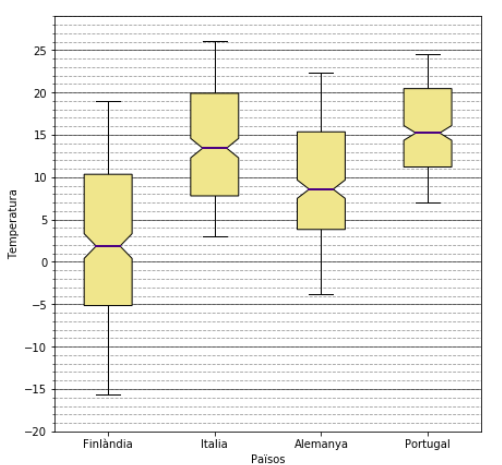
\includegraphics[width=0.5\textwidth]{../img/tempMitjaVariacioPaisos}
	\caption{Temperatures }
	\label{fig-tempMitjaPaisos}
\end{figure}

A més d'analitzar el conjunt de dades també ha estat necessari passar els països a dades numèriques, ja que Scikit-Learn no permet \textit{strings} per entrenar els seus algorismes [19]. Aquesta acció s'havia de fer d'una manera que no convertís les variables en categòriques, és a dir, que l'algorisme no entengués que ser d'un país o d'un altre tenia una relació numèrica. Per fer-ho s'ha utilitzat un mètode de la mateixa llibreria de SciKit-Learn anomenada \textit{get\_dummies}\footnote{\url{Get Dummies: https://bit.ly/2RRSVR9}} que transforma els \textit{string} en un conjunt de variables binàries, per tant si és d'un país, serà un 1 i si no ho és, serà 0.

Un cop sabent que el conjunt de dades era adequat per fer aquestes anàlisis, s'ha començat a escollir i entrenar diversos algorismes de regressió. Dins de la regressió s'ha decidit agafar un conjunt de mètodes que es considerin dins de l'estat de l'art actual en temes de \textit{machine learning}.

\subsubsection{Arbres de Decisió} Els arbres de decisió són models predictius no linears que serveixen per fer tasques de regressió i tasques de classificació. La idea és simple, si es vol predir una classe o resposta Y a partir d'entrades X cal fer créixer un arbre binari. En els nodes d'aquest arbre binari s'aplica un test sobre l'entrada que es consideri més rellevant, per exemple en la figura 2 es comença preguntant sobre la contaminació de CO$_2$. En aquest test es fa una pregunta binària de si o no, si la resposta és si es passarà al fill de la dreta, si la resposta és no, es passarà al fill de l'esquerra. A partir d'aquí, es van fent tests en cada un dels nodes, l'input que s'agafa per formular la pregunta pot variar segons les dades que s'estiguin treballant. Com es mostra a la figura 2 si s'envà cap a l'esquerra, es passa a testejar l'input de les emissions de CH$_4$. A la figura també es pot observar com les prediccions sobre quina és la temperatura final s'acaben fent en arribar a les fulles de l'arbre. Aquestes prediccions vénen donades pel conjunt de totes les preguntes que s'han anat formulant en els seus antecessors [14].
\begin{figure}[!h]
\centering
	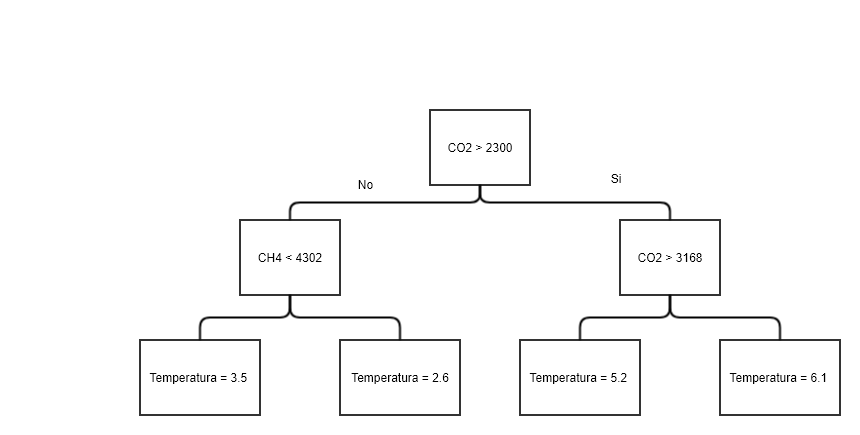
\includegraphics[width=0.5\textwidth]{../img/arbreDecisioSimple}
	\caption{Arbre de Decisió Bàsic}
	\label{fig-DecisionTree}
\end{figure}

Quan hi ha moltes entrades a l'hora d'entrenar l'arbre de decisió, el mateix arbre ha d'escollir quin paràmetre de les entrades cal avaluar primer. Una mala elecció d'aquesta entrada pot comportar que es comenci a fer comprovacions innecessàries, causant un impacte negatiu en l'eficiència de l'entrenament. L'arbre de decisió té diverses estratègies per fer aquesta elecció, però en essència busca quins dels atributs és més rellevant de cara a separar les classes i predir la sortida del problema. Aquesta decisió la fa en cada un dels nodes i va variant fins a arribar a una fulla. Si en aquesta recerca es trobessin dues preguntes sobre dos entrades, que donen la mateixa quantitat d'informació, l'arbre escull una arbitràriament [14].

Per acabar, els arbres de decisions tenen molts paràmetres editables com la seva longitud màxima, el nombre màxim de fulles, el mínim nombre de paràmetres per considerar el node com una fulla... La majoria d'aquests paràmetres limiten el creixement de l'arbre, ja que per defecte creix fins a fer totes les preguntes possibles. Aquests paràmetres són molt importants en l'obtenció de bons resultats. Per exemple, si es para el creixement de l'arbre, en una profunditat que no sigui l'òptima, pot provocar que es descarti gran part de la informació i que l'arbre no encerti en donar la resposta final. També pot passar que es pari l'arbre a una profunditat massa elevada i que es consumeixin recursos sense que s'obtingui un resultat millor [14].

\subsubsection{Support Vector machines}
Support Vector machines o SVM és un mètode d'aprenentatge supervisat que es pot utilitzar per a la classificació i la regressió. Aquest mètode té com a objectiu principal definir una funció $f(x)$ que tingui com a molt una desviació o error per sota d'un límit establert en la creació del mètode. Per exemple, si s'estableix un error igual a 1, es descartaran tots els objectius amb un error superior a 1, i es consideraran tots els que tinguin un valor inferior. Un altre dels seus principals objectius consisteix a trobar un hiperplà de X dimensions, on X és el nombre de variables, que pugui separar òptimament els punts de les diferents classes. Un hiperplà òptim es considera quan aquest es troba a una distància màxima dels punts d'ambdues classes, els punts més pròxims a aquests hiperplans s'anomenen \textit{support vectors}. Aquests punts són la clau en determinar la posició i orientació d'un hiperplà i determinar la distància màxima entre classes [15].

El SVM treballa amb productes sobre punts dins de dimensions definides, així troba les familiaritats entre dos vectors. Els SVM tenen un paràmetre essencial anomenat kernel, que bàsicament són un conjunt de fórmules matemàtiques que defineixen com es processarà les dades que entren com a entrades. Els kernels són els encarregats de modificar el producte de punts establert pel SVM i adaptar-lo al seu espai. Per defecte el SVM té com a kernel el lineal, que limita el producte de punts original en dues dimensions. Si en lloc del lineal s'utilitzes un kernel com el polinòmic, aquest espai acceptaria també combinacions polinòmiques fins a certs graus, aconseguint fer paràboles [15].

A més d'aquests dos, hi ha un de molt utilitzat anomenat Radial Basis Function o RBF. Aquest utilitza un espai limitat per distribucions Gaussianes, en la majoria d'ocasions aquest kernel és el que pot arribar a obtenir els millors resultats [16]. Això és a causa del fet que les funcions Gaussianes són més flexibles a l'hora de reballar amb diferents dimensions d'hiperplà. Per exemple, en la figura 3 es pot veure una petita prova per demostrar el comportament dels tres kernels més utilitzats. Aquí es pot veure clarament com els kernels linears i polinomial no s'adeqüen bé amb un conjunt de dades que varia molt, en canvi el kernel RBF s'ha pogut adaptar millor a aquesta variació i ha pogut traçar una corba amb un error bastant baix.
\begin{figure}[!h]
\centering
	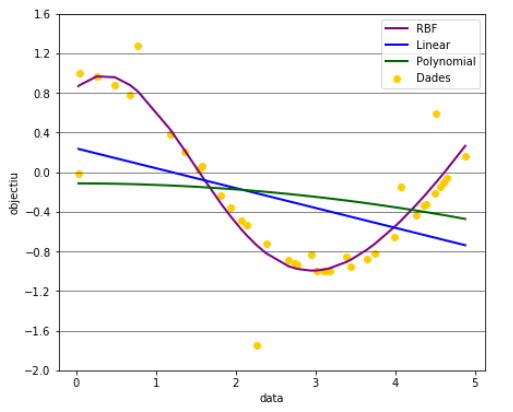
\includegraphics[width=0.5\textwidth]{../img/KernelsSVM}
	\caption{Comparació de kernels SVM}
	\label{fig-KernelsSVM}
\end{figure}

Cada un dels kernels té els seus paràmetres que modifiquen el seu comportament, per exemple, el kernel polinòmic té un anomenat \textit{degree} que modifica el grau del polinomi que s'utilitzarà per trobar el millor hiperplà. En el cas del RBF hi ha dos paràmetres que determinen el seu percentatge d'encerts, aquests son C i \textit{gamma}.
\begin{description}
\item[C:] Com s'ha dit abans, les SVM pretenen aconseguir un marge màxim i tenir un error mínim de classificació. Aquest paràmetre és l'encarregat de determinar a què se li dóna prioritat. Una C elevada, seria correcte si és tingués una funció de regressió que fes bones prediccions amb la majoria de punts amb els quals s'entrena, per tant cal reduir el marge màxim, ja que l'error és petit. En canvi una C petita convé si es té una funció de regressió més simple i que produeix més errors, llavors es necessita augmentar el marge màxim per incloure més punts.
\item[Gamma:] El comportament de SVM és molt sensible a aquest parametre, ja que indica el radi d'influencia que tenen els \textit{support vector} a la resta del conjunt de dades. Per una banda, si aquest paràmetre és molt petit, l'algorisme no podrà entendre la complexitat total del conjunt de dades i es comportaria d'una forma semblant a un kernel linear, ja que aquest paràmetre li indicarà que pot agrupar la majoria d'ells amb el valor dels punts \textit{support vector}. Per l'altra, si és molt gran, es produiria una situació d'overfitting. El rang quedaria limitat al propi \textit{support vector} i no podria agrupar cap dels punts amb ell, per tant també produiria un error molt elevat.
\end{description}

\subsubsection{Random Forest}
El Random Forest és un dels mètodes de ML que s'està utilitzant més en l'actualitat, com els altres dos, es pot utilitzar tant per classificació com per regressió. La idea principal del \textit{random forest} és la de combinar diversos arbres de decisió relacionats entre ells. Es basa en la idea que la combinació de molts algoritmes simples aconsegueix millors resultats que un de sol, encara que aquest sigui molt potent. Com es pot veure a la figura 4, que representa un Random Forest amb dos arbres, el mètode crea dos arbres de decisió i després combina els resultats de cada un d'ells mitjançant el \textit{bagging method} o un altre algoritme segons la implementació que s'esculli [17]. Aquest mètode combina prediccions de múltiples algoritmes per aconseguir una resposta final més exacta. El \textit{bagging} és útil quan hi ha algoritmes amb una variància molt elevada, com els arbres de decisió, i bàsicament aplica el mètode anomenat \textit{bootstrap} a aquests algorismes.\textit{bootstrap} s'encarrega d'agafar un nombre determinat de subconjunts de dades, dins del conjunt, i calcula la mediana del subconjunt. Un cop té totes les medianes agafa la mitjana de totes elles aconseguint el resultat final.
\begin{figure}[!h]
\centering
	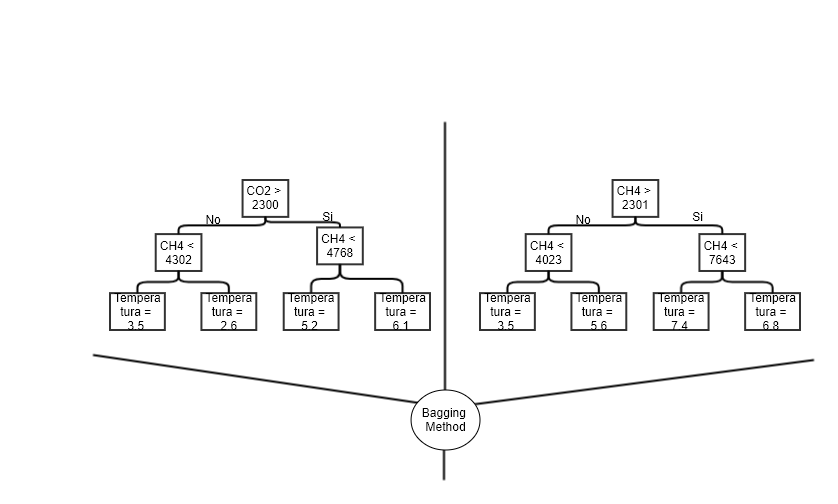
\includegraphics[width=0.5\textwidth]{../img/randomForest}
	\caption{Random Forest amb 2 arbres}
	\label{fig-RandomForest}
\end{figure}

El Random Forest té pràcticament els mateixos paràmetres que un arbre de decisió però amb petites diferències que optimitzen cada una de les decisions preses per l'arbre. Com s'ha dit anteriorment els arbres necessiten escollir quina pregunta s'ha de fer en cada node per aconseguir informació a l'hora de separar les variables. Aquesta situació fa que si s'agrupessin molts arbres junts, tots acabarien sent pràcticament iguals, ja que tots escollirien la mateixa manera de separar. Aquest fet no aportaria una millora molt gran, ja que al final el resultat seria pràcticament el mateix per tots els arbres i a l'hora d'agrupar-los la mitjana acabaria resultant aquell nombre. Per evitar això el Random Forest separa les entrades en subconjunts i cada arbre ha d'escollir de forma aleatòria la millor entrada per separar les dades. Així cada arbre acabarà tenint un subconjunt diferent entrades i els resultats seran més dispersos, que permetrà adaptar-se més a qualsevol conjunt de dades a l'hora de predir [18].

El Random Forest permet editar molts paràmetres entre els quals destaquen:
\begin{description}
\item[N\_estimators:] Permet modificar el nombre d'arbres de decisió abans de començar a aplicar el \textit{bagging method}.
\item[Min\_sample\_leaf:] És igual al dels arbres de decisió i serveix per determinar el mínim nombre de mostres que es necessita per ser una fulla.
\item[Max\_depth:] Determina la profunditat màxima dels arbres de decisió.
\item[Min\_samples\_split:] És igual al dels arbres de decisió i serveix per determinar el mínim nombre de mostres que es necessita per dividir un node.
\end{description}

\subsubsection{Xarxes Neuronals}
Actualment les xarxes neuronals són dels algorismes més prometedors en l'àmbit del \textit{machine learning} o \textit{deep learning}. Destaquen per la seva versatilitat, escalabilitat i una gran potència de còmput. Les més utilitzades, i que han demostrat millors resultats, han sigut les \textit{Multi Layer Perceptron} o MLP. Aquest tipus de xarxes es basen en la combinació de \textit{perceptrons}, una de les arquitectures de xarxes neuronals més simples formada per una capa de \textit{Threshold Logic Unit} o TLU. Al cap i a la fi una MLP està formada per diverses capes de TLU amb una capa destinada a rebre les dades d'entrada, un conjunt de capes internes i una capa destinada a treure les prediccions [18].

Tal com es pot veure a la figura 5 totes les neurones que formen part de la xarxa estan completament interconnectades entre elles, excepte l'última capa que només retorna els resultats. Aquí es pot veure com les capes poden tenir un nombre de neurones diferent, tot i això es recomana acabar amb una sola neurona si al final s'ha de retornar una única predicció. També es pot observar els diferents tipus de capes dins d'una xarxa neuronal simple.
 \begin{figure}[!h]
\centering
	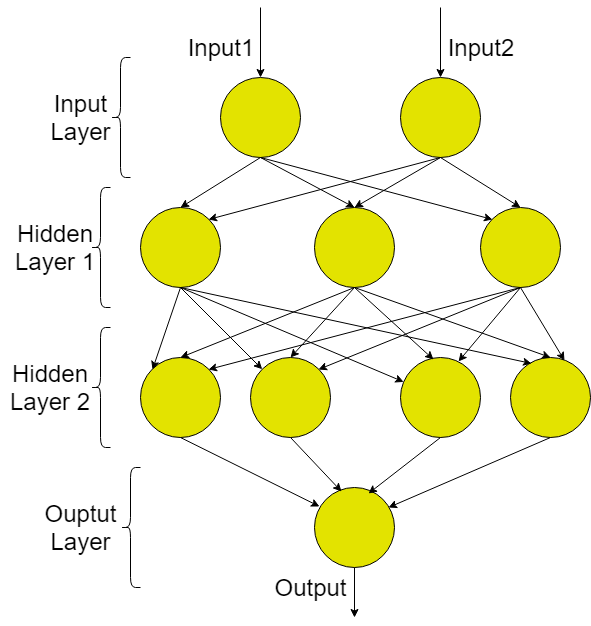
\includegraphics[width=0.5\textwidth]{../img/XarxaNeur}
	\caption{Xarxa Neuronal de 4 capes}
	\label{fig-XarxaNeur}
\end{figure}

Al començament es va decidir utilitzar les xarxes que ofereix la llibreria Scikit-Learn, d'on s'han tret tots els algorismes anteriors, però en aquest hi havia fortes limitacions que no permetien crear una xarxa que no permet la flexibilitat suficient per poder editar tots els hípers-paràmetres i capes que es pretenia en el treball. Per això es va decidir buscar una alternativa millor que pogués demostrar totes aquestes característiques que la fan destacar.

Aquesta alternativa ha acabat sent la llibreria de Keras. Keras treballa sobre TensorFlow, un framework dedicat especialment pel \textit{machine learning} que es troba en l'estat de l'art d'aquest àmbit, però només estableix una capa per sobre d'ell per tal de facilitar la implementació d'algorismes mantenint totes les avantatges del framework. Amb aquesta llibreria sí que s'ha pogut provar diferents models de xarxes amb capes de diferents neurones i amb diferents funcions d'activació [18].

Una xarxa neuronal és molt més extensa d'editar que els altres algorismes, a causa de la seva gran quantitat d'híper-paràmetres i la diversitat entre les combinacions entre ells. En aquest treball no ens hem centrat únicament en les xarxes neuronals, per tant, no ha estat possible explorar totes les possibilitats i variacions de xarxes existents. En aquest cas només s'han contemplat els models seqüencials de Keras, que funcionen sense problemes per tots els casos i amb bons resultats. També s'ha establert una limitació en el nombre de capes per tal de no complicar massa la xarxa i que la complexitat i temps d'entrenament no augmentés massa. A partir d'aquí tota la resta d'híper-paràmetres s'ha deixat sense limitacions [18].

Entre els paràmetres hi ha uns quants que cal destacar per l'afectació que té en el comportament d'una xarxa:
\begin{description}
\item [\textit{Activation}:] Aquest paràmetre és el més rellevant de tots, ja que decideix quan es considera una neurona activada, i quan no. Per exemple es pot establir un llindar i si una neurona el supera, es considera activada, si no es considera desactivada, aquest seria l'activació binaria o \textit{step function}. També hi ha la linear on l'activació és proporcional als entrades o neurones del sistema. Una altra bastant utilitzada és la Relu que té un comportament semblant al linear però considerant com a funció d'activació qualsevol valor positiu superior a 0 [25].
\item[Batch\_size:] És el nombre de mostres que es propagaran al llarg de la xarxa. Per exemple, si es té un conjunt de 1000 dades, però aquest paràmetre és 100, s'aniran agafant subconjunts de 100 i s'aniran propagant per la xarxa.
\item[\textit{Epochs}:] Són el nombre de cops que es propagaran totes les dades per la xarxa. Si es té un batch\_size molt petit i un epoch molt gran és necessitaran moltes iteracions per acabar d'entrenar-la.
\end{description}

\subsubsection{SearchCV}
D'aquests algorismes s'ha fet un entrenament amb els paràmetres per defecte marcats per la llibreria de Scikit-Learn i després s'ha utilitzat dues tècniques, molt utilitzades en l'àmbit del ML per trobar el conjunt de paràmetres més òptim per cada algorisme. Aquestes tècniques tenen com a objectiu esprémer al màxim els algorismes i aconseguir l'aproximació més precisa de la temperatura. Aquestes han estat:
\begin{description}
\item[Grid SearchCV:] Implementa una recerca exhaustiva dels paràmetres editables d'un mètode de predicció. A partir d'aquí el \textit{grid search} crea una quadrícula a on fica tots els paràmetres que es volen modificar i va provant totes les combinacions possibles amb ells fins a completar la taula. Per comprovar quina combinació és millor se li pot passar qualsevol de les fórmules que s'utilitzen per avaluar algorismes, com el MAE o el Mean Squared Error. Un cop fet aquestes anàlisis entrena l'algorisme amb la millor combinació de paràmetres que ha trobat [19].

\item[Randomized SearchCV:] És un mètode molt semblant al \textit{grid search}. També fa una recerca sobre els millors paràmetres, que facin que l'algorisme doni el millor resultat possible. El funcionament és pràcticament igual al \textit{grid search} però les comparacions que fa es fan en un ordre aleatori. Això permet que es puguin provar valors molt elevats sense necessitat de què els recursos necessaris, per fer la recerca, augmentin de forma exponencial [19].


\end{description}
\section{Resultats}
Per aconseguir els millors resultats amb cada un dels algorismes s'han fet proves exhaustives amb el Randomized Search. En el cas de les Xarxes Neuronals no s'ha pogut utilitzar el mateix mètode a causa del fet que no es podia implementar un Grid o Randomized Search que anés creant capes diferents de la xarxa segons avançava... En aquest cas s'ha hagut d'anar provant diferents valors aleatoris i fer una recerca més exhaustiva sobre quines combinacions podien donar millors resultats. Primer es va provar amb capes amb molt poques neurones cada una, després es va provar amb capes de tipus \textit{dropout}, aquestes descarten un número determinat de neurones per evitar que l'algorisme caigui en \textit{l'overfitting}\footnote{Overfitting:      \url{https://bit.ly/2E1IGWJ}}. A més d'això es va provar començar amb capes amb moltes neurones i anar variant en les capes internes fins a arribar a l'última amb una, aquesta última capa sempre s'ha mantingut així ja que donava millors resultats. Un cop trobat la millor combinació de capes i neurones es van fer proves amb diferents maneres d'activació en cada una d'elles, al final la que ha donat millors resultats ha estat la Relu en totes menys en l'última capa que és lineal. Per acabar s'ha dissenyat un GridSearch molt simple que buscava les millors combinacions de batch\_size i de epochs per acabar de perfeccionar la xarxa. 

En la figura 6 es pot veure com s'ha anat comportant la Xarxa Neuronal en cada un dels epochs, es pot veure com, en un inici, la xarxa tenia un MAE molt elevat i a mesura que ha anat aprenent aquest error ha anat disminuint fins arribar als 2.5.
\begin{figure}[!h]
\centering
	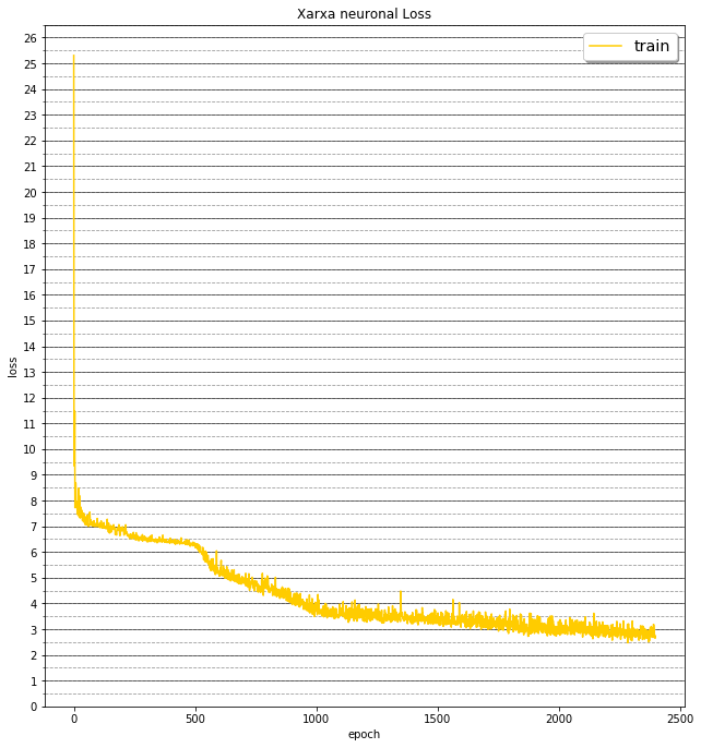
\includegraphics[width=0.5\textwidth]{../img/analisiNN}
	\caption{Comportament Xarxa Neuronal}
	\label{fig-analisiNN}
\end{figure}

En la resta d'algorismes els millors resultats els ha donat la tècnica de Randomized Search. Això s'ha donat a causa del fet que la tècnica pot arribar a paràmetres molt més grans i diversos. El Grid Search no pot fer el mateix pel fet que el Randomized utilitza iteracions de valors aleatoris, dins d'un rang molt més gran de valors. En canvi, el Grid Search està limitat a anar fent proves seqüencialment, començant pels valors més petits i fins a arribar al màxim del rang que s'ha establert. Al cap i a la fi el Grid Search està limitat per la quantitat elevada de càlculs que necessita fer. Per exemple, ficant el mateix nombre de variables, amb el mateix rang de valors en cada una d'elles, per arribar al valor màxim el Grid Search ha de fer X iteracions prèvies (on X pot ser un número molt elevat d'iteracions), en canvi el Randomized ho pot fer a la primera sense passar per totes les anteriors.

Per avaluar l'algorisme hi ha diversos valors que es poden obtenir a partir de la comparació del valor predit i del valor real. En aquest treball s'ha escollit el \textit{Mean Absolut Error}. La principal raó de per què s'ha escollit és perquè et dóna una mitjana a partir de l'error absolut, per tant a l'hora d'interpretar purament l'error aquest valor és perfecte i simple. Un altre avantatge és que et dóna en el mateix rang de les dades que s'estan treballant, per tant acaba sent més fàcil veure les diferències i entendre el valor. A la figura 7 es pot veure una comparativa amb els 4 algorismes analitzats i el millor MAE de cada un. Com es pot veure tots han tingut resultats bastant bons considerant que les temperatures varien dins del rang de 6-7 graus.

\begin{figure}[!h]
	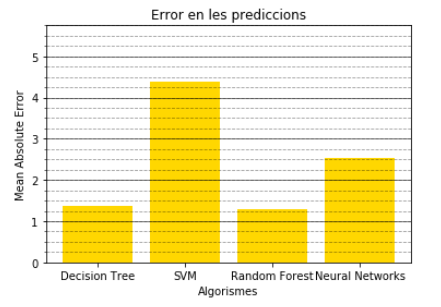
\includegraphics[scale=0.8,center]{../img/comparacioMetricsAlgs}
	\caption{MAE dels mètodes}
	\label{fig-Metrics}
\end{figure}

Com es pot veure a la figura 8 l'algorisme que ha aconseguit aproximar-se més als valors originals ha estat el Random Forest, en canvi el pitjor ha estat l'algorisme de les Support Vector machine.En la figura es veu com la gran majoria d'algorismes s'apropa bastant en les prediccions que fa, però cada algorisme té un comportament bastant diferent de l'hora d'equivocar-se. Per una banda les Xarxes Neuronals fan molt bones prediccions, però manca a l'hora d'endevinar canvis bruscos de temperatura. Les SVM tenen un error constant, sí que és veritat que la tendència de la temperatura la segueixen però en general acostuma a estar uns graus per sobre o per sota, fins i tot en un parell es confon de molts graus.
Per l'altra banda el Random Forest manté bastant la constància amb les temperatures que no varien massa, en canvi sí que falla una mica quan hi ha un canvi brusc de temperatura però manté l'error molt baix. Per l'altra banda els Decision Tree fallen en la gran majoria de prediccions però amb un error baix en tots ells, això fa que el MAE d'ambdós sigui molt semblant, encara que el Random Forest acabi tenint un més baix.

\begin{figure}[!h]
\centering
	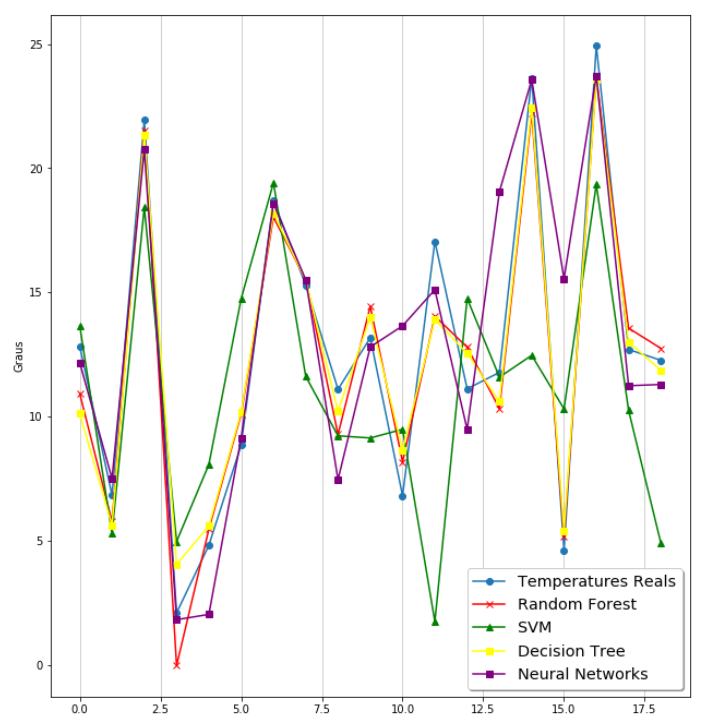
\includegraphics[scale=0.4,center]{../img/comparacioAlgs}
	\caption{Comportament dels mètodes}
	\label{fig-temps}
\end{figure}

\section {Conclusions}
En aquest treball s'ha pogut complir tots els objectius proposats. Els algorismes han donat uns resultats per sobre de l'esperat i el conjunt de dades ha resultat ser adequat per tots els algorismes fins i tot utilitzant diferents frameworks com Scikit-Learn o TensorFlow. Com els algorismes han donat uns resultats amb un error molt baix es pot concloure que sí que hi ha una relació entre les emissions de gasos hivernacle i les temperatures de cada país. En general les aportacions d'aquest treball han sigut:
\begin{itemize}
\item Un conjunt de dades agrupant les temperatures i emissions de gasos hivernacle mensuals, de tots els països Europeus, al llarg de 22 anys.
\item Una comparativa de diversos algorismes de regressió a partir de la predicció feta amb un conjunt de dades amb 7452 registres.
\item Un conjunt d'evidències de què les emissions contaminants dels diversos països afecten directament a la temperatura.
\end{itemize}
Aquest treball ha estat pensat per veure els conceptes més generals de gran part dels àmbits del \textit{machine learning}, com els algorismes principals, tècniques per millorar-los, fórmules per avaluar-los... Però hi ha alguns algorismes que necessiten fer una anàlisi exhaustiu molt extens que podria ocupar tot el treball, com les SVM o les Xarxes Neuronals. Sense aquestes anàlisis és pràcticament impossible trobar la millor combinació de paràmetres i esprémer-los al màxim per aconseguir un error molt baix. Això s'ha notat sobretot en l'extracció de resultats, ja que aquests dos són dels que acostumen a donar millors resultats i en el treball són els que més fallen. Per tant es pot concloure que es pot seguir treballant a partir del que s'ha estat desenvolupant aquí ja que hi ha marge de millora en diversos algorismes.

\section{Treball Futur}
Com a idees per continuar aquest TFG es podria fer la mateixa anàlisi de les dades però en un àmbit mundial en lloc d'europeu. Segurament els resultats siguin encara millors gràcies a un nombre més gran de dades a analitzar. A causa del fet que s'han vist diversos algorismes i s'ha hagut de fer el propi conjunt de dades, no ha sigut possible treballar amb molt de detall algorismes dins de l'estat de l'art del ML, com les SVM i les Xarxes Neuronals. Una línia de treball molt interessant pot ser fer una anàlisi exhaustiu amb algun d'aquests algorismes en un conjunt de dades ja preparat. Si es pot fer exhaustivament, poden sortir resultats molt interessants amb alguns conjunt de dades del canvi climàtic, o també d'un altre àmbit.

Més enllà dels mètodes de Big Data,\textit{machine learning} o aconseguir bons algorismes de regressió, aquest treball també pot acabar sent una bona base perquè apareguin més treballs relacionats amb el canvi climàtic ja que aquest tema es pot aprofitar per aconseguir treballs molt prometedors com, per exemple, muntar uns sensors que detectin quin nivell de contaminació hi ha en un lloc determinat, una aplicació que t'indiqui on va cada residu i fomentar el reciclatge...


\begin{thebibliography}{11}
\bibitem{1}
``World Of Change: Global Temperatures", \textit{NASA}. [En línia]. Disponible a: \url{https://earthobservatory.nasa.gov/world-of-change/DecadalTemp}. [Accedit Gener 23, 2019].
\bibitem{2}
J.Casas, \textit{Introducció al Big Data}. Barcelona, UOC. Pàgines:9-14.
\bibitem{3}
F.Julbe, \textit{Anàlisi de dades massives: Tècniques fonamentals}. Barcelona, UOC.
\bibitem{4}
``Sample Research", \textit{The Standish Group}. [En línia]. Disponible a: \url{https://www.standishgroup.com/sample_research} [Accedit Octubre 4, 2018].
\bibitem{5}
``Scrum Reference Card now available in English and Spanish",  \textit{Agile Methodology}. [En línia]. Disponible a: \url{http://agilemethodology.org/ }. [Accedit Octubre 4, 2018].
\bibitem{6}
``The Complete Guide to Understanding Agile Testing", \textit{QA Symphony}. [En línia].Disponible a: \url{https://www.qasymphony.com/blog/agile-methodology-guide-agile-testing/}. [Accedit Octubre 4, 2018].
\bibitem{7}
``Climate Change: Earth Surface Temperature Data”, \textit{Berkeley Earth}. [En línia]. Disponible a: \url{ https://www.kaggle.com/unitednations/international-greenhouse-gas-emissions}. [Accedit Novembre 9, 2018].
\bibitem{8}
 ``International Greenhouse Gas Emissions”, \textit{United Nations}. [En línia]. Disponible a: \url{ https://www.kaggle.com/unitednations/international-greenhouse-gas-emissions}. [Accedit Novembre 9, 2018].
\bibitem{9}
 ``Land Use, Land-Use Change and Forestry (LULUCF)", \textit{United Nations}. [En línia]. Disponible a: \url{ https://unfccc.int/topics/land-use/workstreams/land-use--land-use-change-lulucf}. [Accedit Novembre 7, 2018].
\bibitem{10}
Federica Pozzi, ``Importancia del recuento del UTCUTS (LULUCF) para el éxito del Acuerdo de París". \textit{Carbon Market Watch}. [En línia]. Disponible a: \url{https://carbonmarketwatch.org/es/2017/07/18/29671/}. [Accedit Novembre 7, 2018].
\bibitem{11}
B.Fornberg, J.Zuev. \textit{The Runge phenomenon and spatially variable shape parameters in RBF interpolation}. University Of Colorado.
\bibitem{12}
 ``Interpolation", \textit{Wikipedia}. [En línia]. Disponible a: \url{https://en.wikipedia.org/wiki/Interpolation#Spline_interpolation}. [Accedit Novembre 10, 2018].
\bibitem{13}
``Encoding Categorical Features", \textit{Scikit-Learn}. [En línia]. Disponible a:\url{https://scikit-learn.org/stable/modules/preprocessing.html#encoding-categorical-features}. [Accedit Desembre 22, 2018].
\bibitem{14}
R. Tibshirani, \textit{Classification and regression trees}. Machine learning Department, Carnegie Mellon University. 2009.
\bibitem{15}
Alex J. Smola, B. Schölkopf, \textit{A tutorial on support vector regression}. RSISE, Australian National University. 2003.
\bibitem{16}
``Kernel Functions-Introduction to SVM Kernel \& Examples", \textit{Data Flair}. [En línia]. Disponible a: \url{https://towardsdatascience.com/the-random-forest-algorithm-d457d499ffcd}. [Accedit Desembre 22, 2018].
\bibitem{17}
L. Breiman, \textit{Random Forests}. Statistics Department, University of California Berkeley. 2001.
\bibitem{18}
A.Géron, \textit{Hands-On Machine Learning with Scikit-Learn \& TensorFlow}. Sebastopol, CA: O’Reilly Media, 2017. Capitol 10.
\bibitem{19}
J. Bergstra i Y. Bengio, \textit{Random search for hyperparameter optimization}. Département d'Informatiques et de recherche opérationelle, Université de Montréal. 2012.

\end{thebibliography}
\clearpage
\newcolumntype{P}[1]{>{\centering\arraybackslash}p{#1}}
\onecolumn
\section{Annex}
\subsection{Comparació individual dels algorismes amb les temperatures reals}

\begin{figure*}[htb!]
    \begin{subfigure}[htb!]{0.5\textwidth}
        	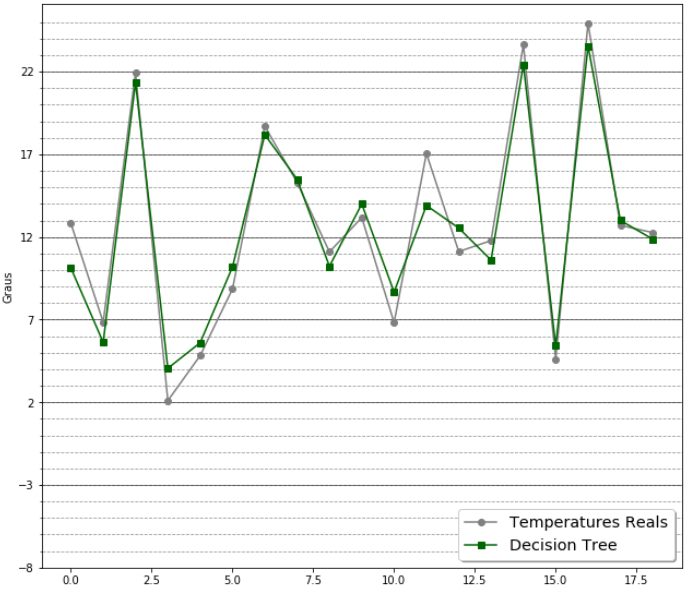
\includegraphics[width=80mm]{../img/decisionTreePredict}
	\caption{Arbre de decisió}
	\label{fig-DT}
    \end{subfigure}
    ~ %add desired spacing between images, e. g. ~, \quad, \qquad, \hfill etc. 
      %(or a blank line to force the subfigure onto a new line)
    \begin{subfigure}[htb!]{0.5\textwidth}
	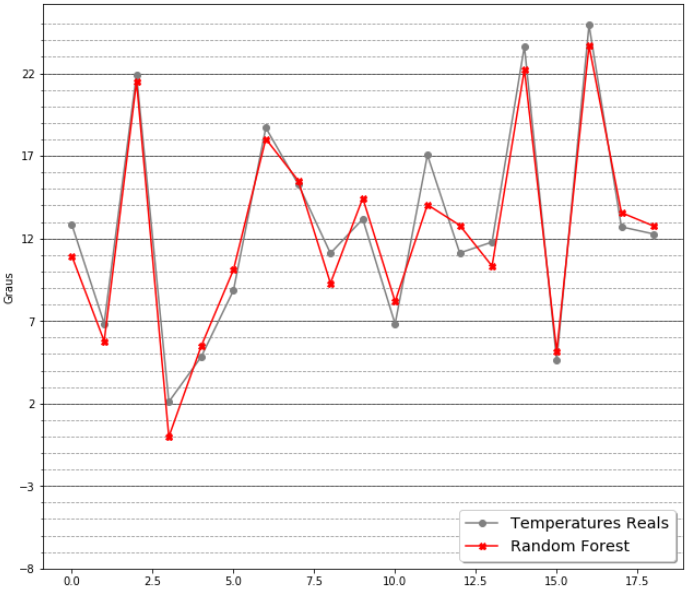
\includegraphics[width=80mm]{../img/randomForestPredict}
	\caption{Random Forest}
	\label{fig-RF}
    \end{subfigure}
	\hfill
 \begin{subfigure}[htb!]{0.5\textwidth}
	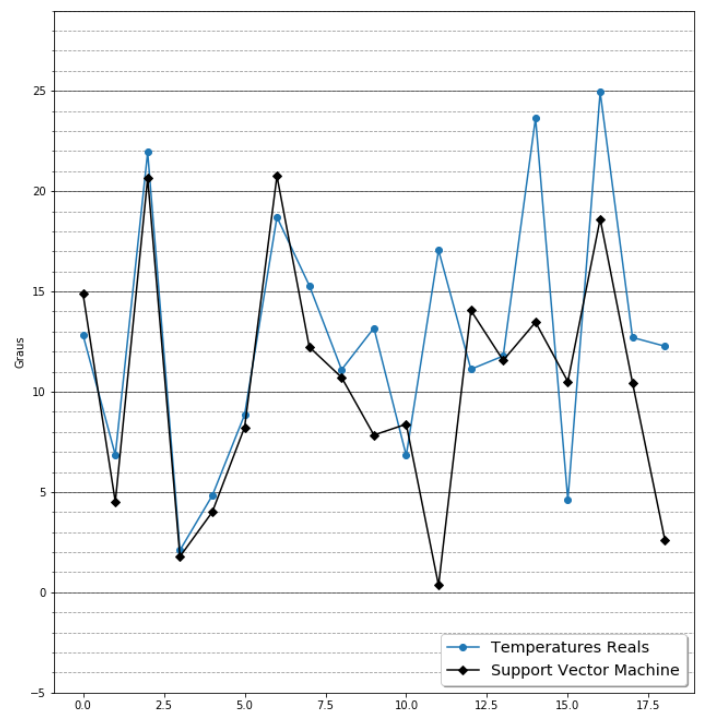
\includegraphics[width=80mm]{../img/SVMPredict}
	\caption{SVM}
	\label{fig-SVM}
    \end{subfigure}
    ~ %add desired spacing between images, e. g. ~, \quad, \qquad, \hfill etc. 
      %(or a blank line to force the subfigure onto a new line)
    \begin{subfigure}[htb!]{0.5\textwidth}
	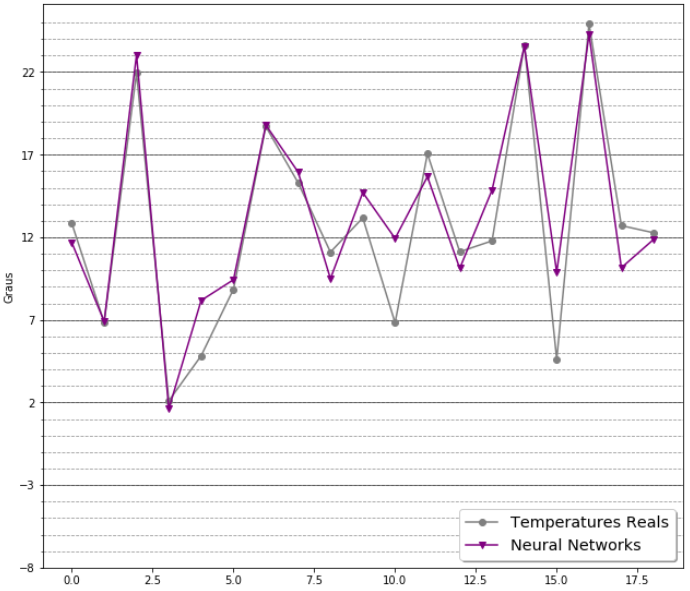
\includegraphics[width=80mm]{../img/XarxesNeurPredict}
	\caption{Xarxes Neuronals}
	\label{fig-NN}
    \end{subfigure}
    \caption{Comparació algorismes}\label{compAlgs}
\end{figure*}
\clearpage
\subsection{Millors híper-parametres per cada algorisme}
\begin{table*}[th]
\caption{Millors combinacions d'híper-parametres}
\begin{center}
\begin{tabular}{  P{3.5cm}| P{10cm} |P{1cm}}
\hline\hline 
\textbf{Algorisme} & \textbf{Híper-parametres} & \textbf{MAE}\\
\hline
Arbre de decisió & max\_depth=475, min\_samples\_leaf=4, min\_samples\_split=23 & 1.36 \\
\hline
Suppor Vector Machine & kernel='rbf', C = 750, gamma = 'scale', tol = 0.06, epsilon=0.6 & 4.38\\
\hline
Random Forest & max\_depth = 172, min\_samples\_leaf = 3, min\_samples\_split = 12, n\_estimators = 1143, random\_state = 28 & 1.28\\
\hline
Xarxes Neuronals & capes=4, Neurones\_1ªCapa=55, Neurones\_2ªCapa=31, Neurones\_3ªCapa=10, Neurones\_4ªCapa=1, epochs=2400, validation\_split = 0.2, batch\_size=84, activation\_3\_primeres\_capes = 'relu', activation\_4ªCapa = 'linear' & 2.28\\
\hline
\hline
\end{tabular}
\end{center}
\end{table*}
\end{document}

